\documentclass[tikz,border=8pt]{standalone}
% Shared look for every TikZ diagram. Load with \input{../../tools/tikz-style.tex}
\usepackage[sfdefault]{roboto}
\usetikzlibrary{arrows.meta, positioning, shapes.geometric, calc, fit, backgrounds}
\definecolor{cblue}{HTML}{4C78A8}
\definecolor{corange}{HTML}{F58518}
\definecolor{cgreen}{HTML}{54A24B}
\definecolor{cred}{HTML}{E45756}
\definecolor{cpurple}{HTML}{B279A2}
\definecolor{cgrey}{HTML}{6B6B6B}
\tikzset{
  every picture/.style={font=\sffamily, line width=1.2pt},
  box/.style={draw=#1, fill=#1!12, rounded corners=4pt, align=center, inner sep=7pt, minimum height=1.1cm},
  box/.default=cgrey,
  arrow/.style={-{Stealth[length=3mm]}, draw=cgrey, line width=1.4pt},
  title/.style={font=\sffamily\bfseries\Large},
  note/.style={font=\sffamily\small, text=cgrey, align=center},
}
\AtBeginDocument{\hyphenpenalty=10000 \exhyphenpenalty=10000}

% A lane graph (after the Lanelet2 routing docs): a two-lane road heading east, cut into lane segments (lanelets).
% Before the junction the left lane must turn left and the right lane goes straight on. Each lanelet is a vertex;
% solid arrows join a lanelet to the one that follows it in the same lane (succeeding); dashed arrows join
% neighbouring lanelets a car may change between (left and right), with a lane-change penalty.
\begin{document}
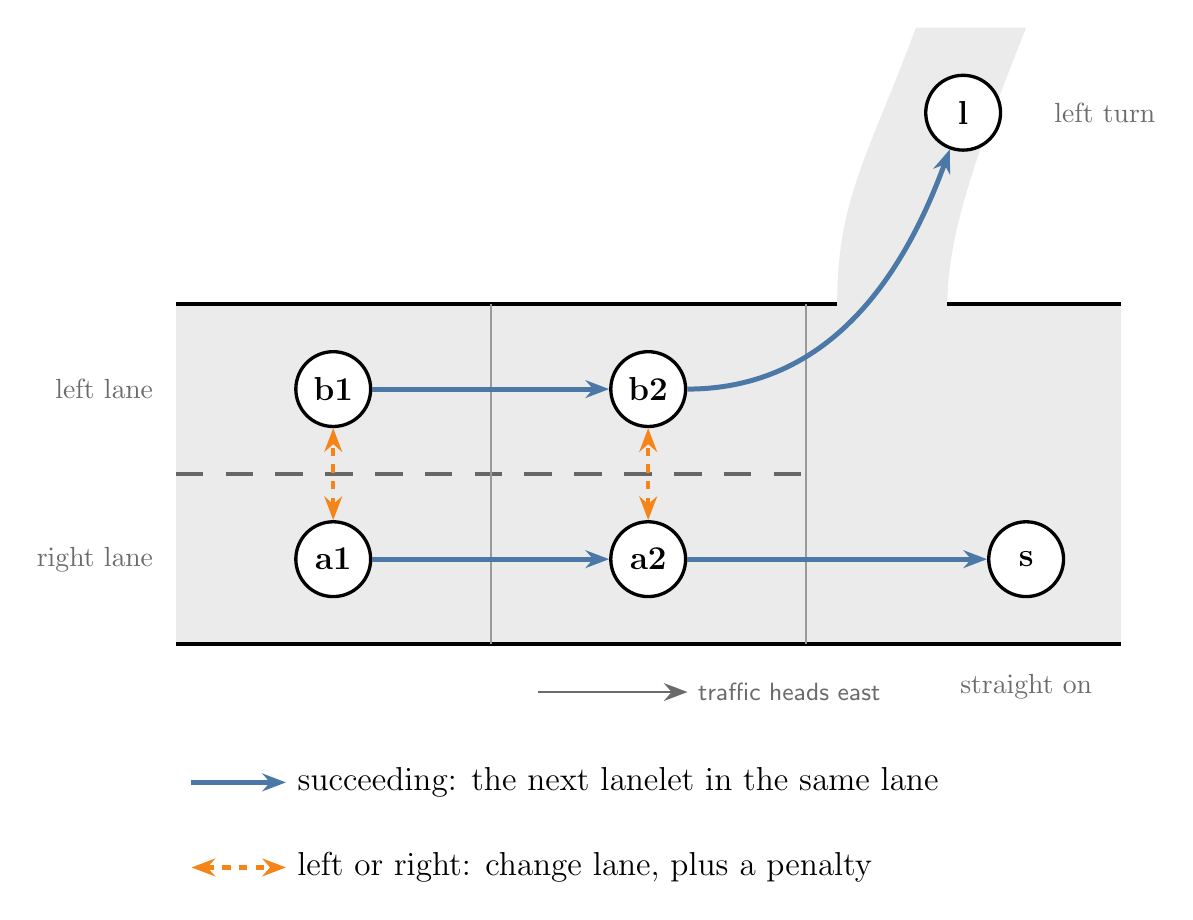
\begin{tikzpicture}[y=1.35cm, every node/.append style={font=\large},
  ll/.style={circle, draw=black, fill=white, minimum size=0.95cm, inner sep=0pt, font=\large\bfseries},
  succ/.style={-{Stealth[length=3mm]}, line width=1.8pt, draw=cblue},
  chg/.style={{Stealth[length=3mm]}-{Stealth[length=3mm]}, line width=1.6pt, draw=corange, dashed}]
  % the road: lanes 1.6 wide, right lane y 0 to 1.6, left lane y 1.6 to 3.2
  \fill[black!8] (0,0) rectangle (12,3.2);
  \fill[black!8] (8.4,3.2) .. controls (8.4,4.2) and (8.8,4.6) .. (9.4,5.8) -- (10.8,5.8) .. controls (10.1,4.5) and (9.8,3.8) .. (9.8,3.2) -- cycle;
  \draw[black, line width=1.5pt] (0,0) -- (12,0);
  \draw[black, line width=1.5pt] (0,3.2) -- (8.4,3.2);
  \draw[black, line width=1.5pt] (9.8,3.2) -- (12,3.2);
  \draw[black!60, line width=1.2pt, dash pattern=on 10pt off 8pt] (0,1.6) -- (8,1.6);
  \draw[black!40, line width=0.8pt] (4,0) -- (4,3.2);
  \draw[black!40, line width=0.8pt] (8,0) -- (8,3.2);
  \draw[cgrey, line width=1pt, -{Stealth[length=3mm]}] (4.6,-0.45) -- (6.5,-0.45) node[right, note] {traffic heads east};
  \node[note, font=\normalsize, anchor=east] at (-0.15,2.4) {left lane};
  \node[note, font=\normalsize, anchor=east] at (-0.15,0.8) {right lane};
  % the lanelets as vertices
  \node[ll] (a1) at (2,0.8) {a1};
  \node[ll] (b1) at (2,2.4) {b1};
  \node[ll] (a2) at (6,0.8) {a2};
  \node[ll] (b2) at (6,2.4) {b2};
  \node[ll] (s) at (10.8,0.8) {s};
  \node[ll] (l) at (10.0,5.0) {l};
  \draw[succ] (a1) -- (a2);
  \draw[succ] (b1) -- (b2);
  \draw[succ] (a2) -- (s);
  \draw[succ] (b2) to[out=0, in=-110] (l);
  \draw[chg] (a1) -- (b1);
  \draw[chg] (a2) -- (b2);
  \node[note, font=\normalsize, align=left] at (11.8,5.0) {left turn};
  \node[note, font=\normalsize] at (10.8,-0.4) {straight on};
  % legend
  \draw[succ] (0.2,-1.3) -- (1.4,-1.3) node[right, black] {succeeding: the next lanelet in the same lane};
  \draw[chg] (0.2,-2.1) -- (1.4,-2.1) node[right, black] {left or right: change lane, plus a penalty};
\end{tikzpicture}
\end{document}
